 \documentclass{article}

\usepackage[utf8]{inputenc}
\usepackage{amsthm}
\usepackage{amssymb}
\usepackage{mathtools}
\usepackage{graphicx}
\usepackage{mdframed}
\usepackage{float}
\usepackage[top=0.75in, bottom=0.75in, left=0.75in, right=0.75in]{geometry}
\usepackage{gauss}

\usepackage{array}
\allowdisplaybreaks

\makeatletter
\newcounter{elimination@steps}
\newcolumntype{R}[1]{>{\raggedleft\arraybackslash$}p{#1}<{$}}
\def\elimination@num@rights{}
\def\elimination@num@variables{}
\def\elimination@col@width{}
\newenvironment{elimination}[4][0]
{
    \setcounter{elimination@steps}{0}
    \def\elimination@num@rights{#1}
    \def\elimination@num@variables{#2}
    \def\elimination@col@width{#3}
    \renewcommand{\arraystretch}{#4}
    \start@align\@ne\st@rredtrue\m@ne
}
{
    \endalign
    \ignorespacesafterend
}
\newcommand{\step}[2]
{
    \ifnum\value{elimination@steps}>0\sim\quad\fi
    \left[
        \ifnum\elimination@num@rights>0
            \begin{array}
            {@{}*{\elimination@num@variables}{R{\elimination@col@width}}
            |@{}*{\elimination@num@rights}{R{\elimination@col@width}}}
        \else
            \begin{array}
            {@{}*{\elimination@num@variables}{R{\elimination@col@width}}}
        \fi
            #1
        \end{array}
    \right]
    & 
    \begin{array}{l}
        #2
    \end{array}
    \addtocounter{elimination@steps}{1}
}
\makeatother

\DeclarePairedDelimiter{\abs}{\lvert}{\rvert}
\DeclarePairedDelimiter{\norm}{\lvert \lvert}{\rvert \rvert}

\newtheoremstyle{break}% name
  {}%         Space above, empty = `usual value'
  {}%         Space below
  {\itshape}% Body font
  {}%         Indent amount (empty = no indent, \parindent = para indent)
  {\bfseries}% Thm head font
  {.}%        Punctuation after thm head
  {\newline}% Space after thm head: \newline = linebreak
  {}%         Thm head spec

\newtheorem{Def}{Definition}[section]

\theoremstyle{break}

\newtheorem{innerEx}{Exempel}[section]
\newtheorem{sats}{Sats}[section]
\newtheorem{Rem}{Anmärkning}[]

\newenvironment{Ex}
{\begin{mdframed} \begin{innerEx} \vspace{3pt}}
{\vspace{3pt} \end{innerEx} \end{mdframed}}  

\newenvironment{bevis}
{\begin{mdframed} \begin{proof} \vspace{3pt}}
{\vspace{3pt} \end{proof} \end{mdframed}}

\title{
	 Linjär Algebra\\
	 Föreläsning 6
    \author{Erik Sjöström}
}
\begin{document}
\maketitle

\section{Determinanter} % (fold)
\label{sec:matrisvektorprodukt}

En determinant för en matris $\textbf{A}_{n \times n}$ är en funktion som ordnar ett tal till \textbf{A}.
\begin{Def}
    Determinanten för en $(2 \times 2)$-matris $\mathbf{A} = \begin{bmatrix} a_{11}&a_{12}\\a_{21}&a_{22} \end{bmatrix}$:
    \[
        \mathbf{det}(\mathbf{A}) = \begin{vmatrix} a_{11}&a_{12}\\a_{21}&a_{22} \end{vmatrix} = a_{11} \cdot a_{22} - a_{21} \cdot a_{22}
    \]
\end{Def}
\begin{Ex}
    \begin{align*}
    &\mathbf{A} = \begin{bmatrix} \frac{1}{2}&1\\1&0 \end{bmatrix} &\mathbf{det}(\mathbf{A}) = \frac{1}{2} \cdot 0 - 1 \cdot 1 = -1
    \end{align*}
\end{Ex}

\begin{Ex}
    \begin{align*}
    &\mathbf{B} = \begin{bmatrix} 2&4\\1&2 \end{bmatrix} & \mathbf{det}(\mathbf{B}) = 2 \cdot 2 - 1 \cdot 4 = 0
    \end{align*}
\end{Ex}

\section{Geometrisk tolkning} % (fold)
\label{sec:geometrisk_tolkning}
\begin{sats}
    Låt $\mathbf{A}_{2 \times 2}$ = $\begin{bmatrix} \vec{a_1} &\vec{a_2} \end{bmatrix}$ där $\vec{a_1}$, $\vec{a_2}$ är vektorer i $\mathbb{R}^2$. Arean av parallellogrammet som spänns upp av $\vec{a_1}$ och $\vec{a_2}$ ges av $\abs{\mathbf{det}(\mathbf{A})}$
    \begin{center}
        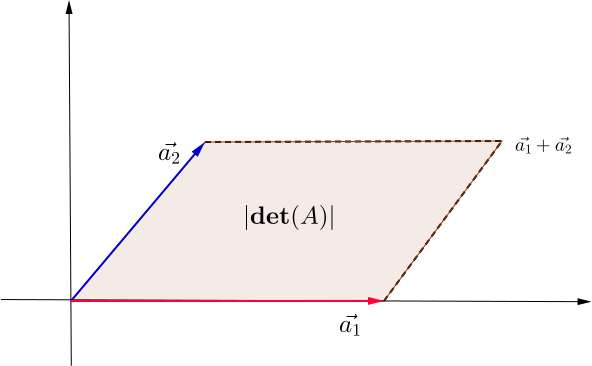
\includegraphics[scale=0.5]{areagram.png}
    \end{center}
\end{sats}

\begin{Ex}
    \begin{align*}
    &\mathbf{A} = \begin{bmatrix} 0.5&1\\1&0 \end{bmatrix} &\mathbf{det}(\mathbf{A}) = 0.5 \cdot 0 - 1 \cdot 1 = -1
    \end{align*}
    \begin{center}
        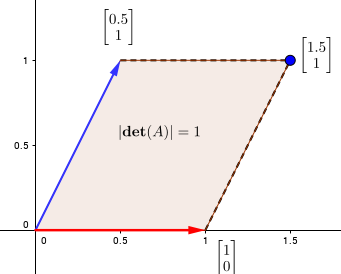
\includegraphics[scale=0.5]{areaex1.png}
    \end{center}
\end{Ex}

\begin{Ex}
    \begin{align*}
    &\mathbf{B} = \begin{bmatrix} 2&4\\1&2 \end{bmatrix} & \mathbf{det}(\mathbf{B}) = 2 \cdot 2 - 1 \cdot 4 = 0
    \end{align*},
    \begin{center}
        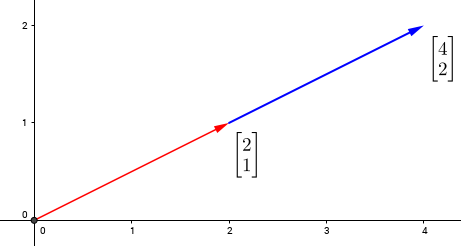
\includegraphics[scale=0.5]{areaex2.png}
    \end{center}
    Kolumnvektorerna i \textbf{B} är pararella:
    \[
        \begin{bmatrix} 4\\2 \end{bmatrix} = 2 \begin{bmatrix} 2\\1 \end{bmatrix}
    \]
    Så arean blir följaktligen noll.
\end{Ex}
\begin{bevis}
\textbf{ Sats 1.1:}
    \begin{center}
        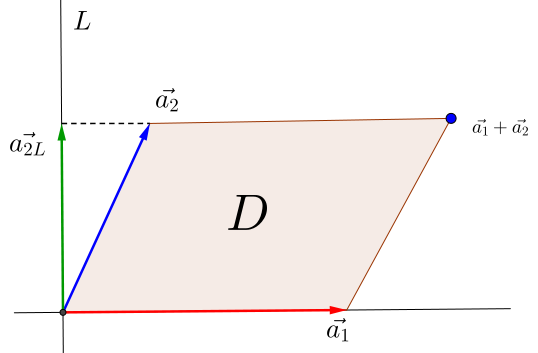
\includegraphics[scale=0.5]{bevis.png}
    \end{center}
    \begin{itemize}
        \item Inför en linje $L$ ortogonal mot $\vec{a_1}$
        \begin{itemize}
            \item Riktningsvektor för $L$: $\vec{v} = \begin{bmatrix} -a_{21}\\a_{11} \end{bmatrix}$
        \end{itemize}
    \end{itemize}
    
    Hur kom vi fram till att $\vec{v} = \begin{bmatrix} -a_{21}\\a_{11} \end{bmatrix}$?\\
    Vi har:
    \[
        a_1 = \begin{bmatrix} a_{11}\\a_{21} \end{bmatrix}
    \]
    Vi vill att:
    \[
         \vec{v} \cdot \vec{a_1} = 0
     \]
     Eftersom då är den ortogonal (definition av skalärprodukt).\\
     Med vårt val av $\vec{v}$ får vi:
    \[
        \vec{v} \cdot \vec{a_1} = -a_{21} \cdot a_{11} + a_{21} \cdot a_{11} = 0
    \]
    \begin{itemize}
        \item Låt $\vec{a_{2L}}$ vara den ortogonala projektionen av $\vec{a_2}$ på linjen $L$
    \end{itemize}
    Arean $D$ blir då:
    \begin{align*}
    D = \mbox{ basen } \cdot \mbox{ höjden } &= \norm{\vec{a_1}} \cdot \norm{\vec{a_{2L}}} = \norm{\vec{a_1}} \cdot \frac{\abs{\vec{a_2} \cdot \vec{v}}}{\norm{\vec{v}}} = \sqrt{a_{11}^2 + a_{21}^2} \cdot \frac{\abs{\vec{a_2} \cdot \vec{v}}}{\sqrt{(-a_{21})^2 + a_{11}^2}} \\
    &= \abs{\vec{a_2} \cdot \vec{v}} = \abs{\begin{bmatrix} a_{12}\\a_{22} \end{bmatrix} \cdot \begin{bmatrix} -a_{21}\\a_{11} \end{bmatrix}} = \abs{a_{12} \cdot (-a_{21}) + a_{22} \cdot a_{11}} \\
    &= \abs{a_{11} \cdot a_{22} - a_{21} \cdot a_{12}} = \abs{\mathbf{det}(\mathbf{A})}
    \end{align*}
\end{bevis}
\noindent
\paragraph
- När blir $\mathbf{det}(\mathbf{A})$: $<0$, $>0$, och $=0$?\\
Vi har från beviset att:
\[
    \mathbf{det}(\mathbf{A}) = \vec{a_2} \cdot \vec{v}
\]
Och detta vet vi (från definitionen av skalärprodukt) är lika med:
\[
    \norm{\vec{a_2}} \cdot \norm{\vec{v}} \cdot \cos(\alpha)
\]
Vi ser då att:
\begin{itemize}
    \item $>0$ om $\alpha$ spetsig
    \item $<0$ om $\alpha$ trubbig
    \item $=0$ om $\vec{v}$, $\vec{a_2}$ är ortogonala
\end{itemize}

\section{Orientering} % (fold)
\label{sec:orientering}
Två vektorer $\vec{u}$, $\vec{v}$ (ej parallella) i $\mathbb{R}^2$ (planet) är högerorienterade om den kortaste vägen att vrida $\vec{u}$ till $\vec{v}$ så att $\vec{u}$ får samma riktning som $\vec{v}$ är moturs, är den kortaste vägen istället medurs så är de vänsterorienterade.

\begin{Ex}
    \textbf{Högerorienterat}:
    \begin{center}
        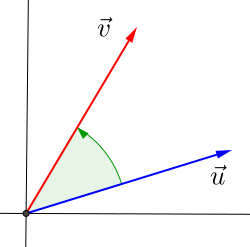
\includegraphics[scale=0.5]{hoger.png}
    \end{center}
    \textbf{Vänsterorienterat}:
    \begin{center}
        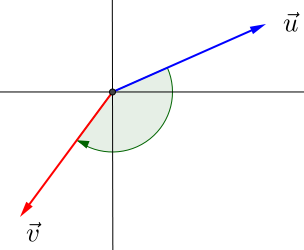
\includegraphics[scale=0.5]{vanster.png}
    \end{center}
\end{Ex}
\paragraph
- Låt $\mathbf{A} = \begin{bmatrix} \vec{a_1}&\vec{a_2} \end{bmatrix}$ ($\vec{a_1}$, $\vec{a_2}$ vektorer i $\mathbb{R}^2$)\\
\textbf{Om} ($\vec{a_1}$, $\vec{a_2}$) är \textbf{högerorienterade} så är vinkeln mellan $\vec{a_{2L}}$ och $\vec{a_2}$ \textbf{spetsig}, och $\mathbf{det}(\mathbf{A}) > 0$\newline
\textbf{Om} ($\vec{a_1}$, $\vec{a_2}$) är \textbf{vänsterorienterade} så är vinkeln mellan $\vec{a_{2L}}$ och $\vec{a_2}$ \textbf{trubbig}, och $\mathbf{det}(\mathbf{A}) < 0$
% section orientering (end)

\section{Determinant för ($3 \times 3$)} % (fold)
\label{sec:determinant_f_r_}
\begin{Def}
    \[
        \mathbf{det}(\mathbf{A}) = \begin{vmatrix} a_{11}&a_{12}&a_{13}\\a_{21}&a_{22}&a_{23}\\a_{31}&a_{32}&a_{33} \end{vmatrix} = a_{11} \begin{vmatrix} a_{21}&a_{23}\\a_{32}&a_{33} \end{vmatrix} - a_{12} \begin{vmatrix} a_{21}&a_{23}\\a_{31}&a_{33} \end{vmatrix} + a_{13} \begin{vmatrix} a_{21}&a_{22}\\a_{31}&a_{32} \end{vmatrix}
    \]
\end{Def}
\begin{Ex}
    Beräkna:
    \begin{align*}
    \begin{vmatrix} 1&0&2\\1&3&1\\-2&0&5 \end{vmatrix} &= 1 \cdot \begin{vmatrix} 3&1\\0&5 \end{vmatrix} - 0 \cdot \begin{vmatrix} 1&1\\-2&5 \end{vmatrix} + 2 \cdot \begin{vmatrix} 1&3\\-2&0 \end{vmatrix} \\
    &= 1 \cdot (3 \cdot 5 - 0 \cdot 1) - 0 \cdot (1 \cdot 5 - (-2) \cdot 1) + 2 \cdot (1 \cdot 0 - (-2) \cdot 3) \\
    &= 15 + 12 = 27
    \end{align*}
\end{Ex}
\begin{Ex}
    Minnesregel för kryssprodukt.\\
    Låt:
    \begin{align*}
    &\vec{u} = \begin{bmatrix} u_1\\u_2\\u_3 \end{bmatrix}, 
    &&\vec{v} = \begin{bmatrix} v_1\\v_2\\v_3 \end{bmatrix}, 
    &&&\vec{e_x} = \begin{bmatrix} 1\\0\\0 \end{bmatrix}, 
    &&&&\vec{e_y} = \begin{bmatrix} 0\\1\\0 \end{bmatrix}, 
    &&&&&\vec{e_z} = \begin{bmatrix} 0\\0\\1 \end{bmatrix}
    \end{align*}
    Kryssprodukten $\vec{u} \times \vec{v}$ går då att lösa på detta vis:
    \begin{align*}
    \vec{u} \times \vec{v} &= \begin{vmatrix} \vec{e_x}&\vec{e_y}&\vec{e_z}\\u_1&u_2&u_3\\v_1&v_2&v_3 \end{vmatrix} = \vec{e_x} \begin{vmatrix} u_2&u_3\\v_2&v_3 \end{vmatrix} - \vec{e_y} \begin{vmatrix} u_1&u_3\\v_1&v_3 \end{vmatrix} + \vec{e_z} \begin{vmatrix} u_1&u_2\\v_1&v_2 \end{vmatrix}\\
    &= \vec{e_x} \cdot (u_2 \cdot v_3 - v_2 \cdot u_3) - \vec{e_y} \cdot (u_1 \cdot v_3 - v_1 \cdot u_3) + \vec{e_z} \cdot (u_1 \cdot v_2 - v_1 \cdot u_2)\\
    &= \begin{bmatrix} u_2v_3 - v_2u_3\\u_3v_1 - v_3u_1\\u_1v_2 - v_1u_2 \end{bmatrix}
    \end{align*}
\end{Ex}
% section determinant_f_r_ (end)

\section{Geometrisk tolkning} % (fold)
\label{sec:geometrisk_tolkning}
Volymen av en parallellepiped med kanterna:
\begin{align*}
 &\vec{a_1} = \begin{bmatrix} a_{11}\\a_{21}\\a_{31} \end{bmatrix}
 &&\vec{a_2} = \begin{bmatrix} a_{21}\\a_{22}\\a_{23} \end{bmatrix}
 &&\vec{a_3} = \begin{bmatrix} a_{31}\\a_{32}\\a_{33} \end{bmatrix}
 \end{align*}
 Ges av absolutbeloppet av:
 \[
     \vec{a_1} \cdot (\vec{a_2} \times \vec{a_3}) = \mathbf{det}(\begin{bmatrix} \vec{a_1}&\vec{a_2}&\vec{a_3} \end{bmatrix})
 \]
\begin{center}
    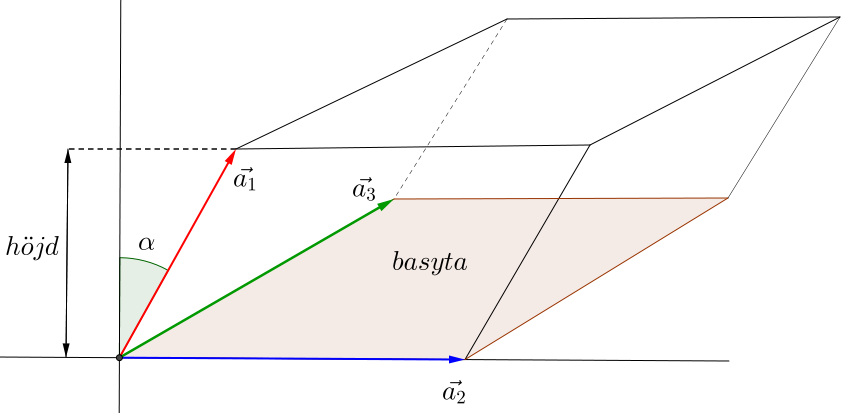
\includegraphics[scale=0.5]{epiped.png}
\end{center}
\begin{align*}
\mbox{Volymen V = basytan }\cdot\mbox{ höjden } &= \norm{\vec{a_2} \times \vec{a_3}} \cdot \norm{\vec{a_1}} \cdot \cos(\alpha) = \vec{a_1} \cdot (\vec{a_2} \times \vec{a_3})
\end{align*}
\begin{align*}
\vec{a_1} \cdot (\vec{a_2} \times \vec{a_3}) = \vec{a_1} \cdot 
\begin{bmatrix} 
\begin{vmatrix} a_{22}&a_{23}\\a_{32}&a_{33} \end{vmatrix} \\
- \begin{vmatrix} a_{21}&a_{23}\\a_{31}&a_{33} \end{vmatrix} \\
\begin{vmatrix} a_{21}&a_{22}\\a_{31}&a_{32} \end{vmatrix}
\end{bmatrix} = a_{11} \cdot \begin{vmatrix} a_{22}&a_{23}\\a_{32}&a_{33} \end{vmatrix} - a_{12} \cdot \begin{vmatrix} a_{21}&a_{23}\\a_{31}&a_{33} \end{vmatrix} + a_{13} \cdot \begin{vmatrix} a_{21}&a_{22}\\a_{31}&a_{32} \end{vmatrix} = \mathbf{det}(\mathbf{A})
\end{align*}
\textbf{det}(\textbf{A}) =
\[
\begin{cases}
    \mbox{V om } (\vec{a_1},\vec{a_2},\vec{a_3}) \mbox{ är högerorienterade}\\
    \mbox{-V om } (\vec{a_1},\vec{a_2},\vec{a_3}) \mbox{ är vänsterorienterade}
\end{cases}
\]
% section geometrisk_tolkning (end)

\section{Orientering} % (fold)
\label{sec:orientering}

Vektortrippeln ($\vec{u}$, $\vec{v}$, $\vec{w}$) i den ordningen (i $\mathbb{R}^3$)är högerorienterade om vektorerna $\vec{u}$ och $\vec{v}$ är högerorienterade i det plan som spänns upp av $\vec{u}$ och $\vec{v}$ sedda från spetsen av $\vec{w}$
\begin{Ex}
    \textbf{Högerorientering}:
    \begin{center}
        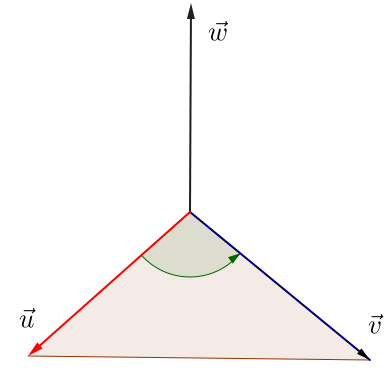
\includegraphics[scale=0.5]{hoger3.png}
    \end{center}
\end{Ex}
\begin{Ex}
    \textbf{Vänsterorienterat}:
    \begin{center}
        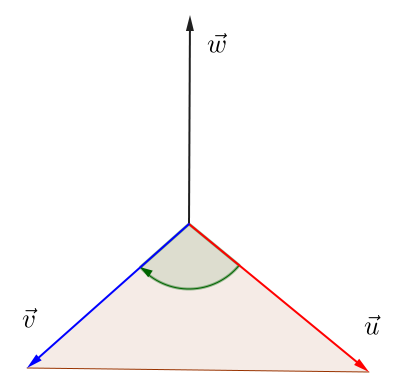
\includegraphics[scale=0.5]{vanster3.png}
    \end{center}
\end{Ex}
% section orientering (end)
\end{document}
